
\chapter{Guide d'utilisateur}
\label{annexe:B}

% Si l'option \verb@hypertexte@ est déclarée, on peut obtenir des liens avec
% la commande \verb@autoref@. Par exemple:
% \begin{center}
% Le \autoref{ch:chapitre-1} est placé avant l'\autoref{annexe:B}.
% \end{center}
% Ceci est à comparer à
% \begin{center}
% Le chapitre~\ref{ch:chapitre-1} est placé avant l'annexe~\ref{annexe:B}.
% \end{center}



\section{Introduction}
L'objectif du logiciel est d'utiliser un ensemble de méthode de convergence de type Newton sur la
librairie MGH au sein de Scilab. 
\begin{equation}
\min_{x\in \mathbb{R}^n} f(x)^Tf(x)
\end{equation}
où $f\in \mathbb{R}^n \rightarrow \mathbb{R}^m$  et $F(x)=\nabla (f(x)^Tf(x))$\\
Pour avoir une résolution des systèmes linéaires $Ax=b$ efficace, nous utilisons une décomposition de Cholesky modifiée
et une résolution du package LAPACK en fortran. Ainsi nous avons dû créer une interface Scilab-Fortran. 
L'ensemble des méthodes, la recherche linéaire et opérations classiques restent sous Scilab.


\section{Installation}


Télécharger le fichier d'archive {\tt Toolboxtapenade.rar} sur\\ \url{http://pages.usherbrooke.ca/rcotte/wp-includes/memoire/} et l'extraire. \`A l'intérieur se trouvent 5 dossiers.

\begin{description}
  \item[Caml] \hfill \\
Mes travaux sur la différentiation automatique avec caml.

  \item[Codescilab] \hfill \\
Pour faire fonctionner le code sous scilab.

  \item[Fonctions] \hfill \\
Ensemble des fonctions à différentier. Ces fichiers sont les originaux; ils proviennent du site :
\url{http://www.netlib.org/uncon/data/}. Avant de les différentier avec Tapenade, des modifications sont faites.

  \item[Librairie] \hfill \\
Contient l'ensemble des librairies pour toutes les fonctions et tous les modes, compilées par gfortran. Il
s'agit de {\tt .o}. Ce sont ces fichiers qu'il faudra recompiler sous scilab si l'on modifie les fonctions. 
Apr\`es avoir exécuté le main.sce dans Codescilab, on pourra directement initialiser les librairies de chaque
probl\`eme grâce à la fonction :\\
{\tt initlib(<Numéro du probl\`eme>);} qui contient notamment : \\
{\tt l=ilib\_for\_link(<Nom de la fonction>,[<Nom du fichier>],[],'f');}\\

  \item[Librairiescilab] \hfill \\
Les libraires créées par la commande {\tt initlib(<Numéro du probl\`eme>);}
se trouvent dans ce dossier. Les fichiers sont de la forme {\tt lib*.so}. Ils vont permettre l'exécution
dans scilab. Une fois qu'ils sont créés, il suffit de les "linker" avec \\
{\tt initlink(<Numéro du probl\`eme>);}\\

  \item[tapenade] \hfill \\
Dossier contenant les fonctions modifiées et un Makefile permettant de créer et compiler le code adjoint
pour chaque fonction.
\end{description}

Pour l'installation suivre les instructions qui se trouvent dans le README.





\section{Comment l'utiliser ?}

Le dossier {\tt Codescilab} contient un fichier {\tt main.sce}, dont il faut changer la variable {\tt path} par le répertoire courant. 
Ensuite, le {\tt main.sce} peut s'exécuter dans scilab sous n'importe quel répertoire. Pour utiliser
les fonctions principales, il suffira seulement d'initialiser le {\it link} au problème avec :\\
{\tt -->initlink(<Numéro du probl\`eme>);}\\



\section{Les fonctions principales}



\rule{\linewidth}{1pt}
\begin{description}
  \item[Fonction d'initialisation] \hfill \\
 {\tt function [n,m,x0,funcname] = initftap(nprog)} \\
Permet d'initialiser les valeurs de {\tt n}, {\tt m}, {\tt x0} données par les routines de LAPACK. Initialise aussi 
le nom de la fonction.
  \item[Paramètres] \hfill \\
\begin{tabular}{lll}
{\tt x0}&:&initialisation de {\tt x0} par la librairie de MGH de taille {\tt n}.\\
{\tt n}&:&initialisation de {\tt n}, taille de {\tt x0}.\\
{\tt m}&:&initialisation de {\tt m}, nombre de composantes de {\tt f}\\
{\tt nprog}&:&numéro du problème, {\tt nprog} $\in [1,\ 35]$ \\ %\lbbbrack 1, \rbbbrack \\
{\tt funcname}&:& contient le nom de la fonction.\\
\end{tabular}
\end{description}
\paragraph{Exemple}{}{\tt initftap}\\
{\tt -->initlink(1)} //Créer le lien pour la librairie\\
{\tt -->[n,m,x0,funcname] = initftap(1)} //initialise les variables pour le problème de Rosenbrock\\
{\tt  funcname  =  rose   \\
 x0  =\\
  - 1.2  \\
    1.   \\
 m  =  2. \\ 
 n  =  2.\\}\\


\begin{description}
  \item[Appel des fonctions standards] \hfill \\
{\tt f=FTF(x,n,m)}\\
{\tt g=G(x,n,m)}\\
{\tt h=H(x,n,m)}\\
{\tt n2d=N2d(x,n,m,d1)}\\
{\tt n2dd=N2dd(x,n,m,d1,d2)}\\
{\tt n3dd=N3dd(x,n,m,d1,d2)}\\
{\tt n3ddd=N3ddd(x,n,m,d1,d2,d3)}\\
Voici l'ensemble des fonctions de base qui permet de calculer les dérivées des fonctions avec 
un coût économique.
  \item[Paramètres] \hfill \\
\begin{tabular}{lll}
{\tt x}&:&variable de décision.\\
{\tt n}&:&taille de {\tt x}.\\
{\tt m}&:&nombre de composantes de {\tt f}, il y a en général des restrictions\\
&& sur {\tt m} par rapport à {\tt n}. Par exemple {\tt m=n}.\\
{\tt d1},{\tt d2},{\tt d3}&:&vecteur colonne de la même taille que {\tt x}.\\
{\tt f}& :& valeur de la fonction objectif en {\tt x}, {\tt f} $\in \mathbb{R}$.\\
{\tt g}& :& valeur du gradient en {\tt x}, {\tt g} $\in \mathbb{R}^n$.\\
{\tt h}& :& valeur du hessien en {\tt x}, {\tt h} $\in \mathbb{R}^{n\times n}$.\\
{\tt n2d}&:& calcule $\nabla^2 F(x)\cdot d_1$, {\tt n2d} $\in \mathbb{R}^{n\times n}$. \\
{\tt n2dd}&:& calcule $\nabla^2 F(x)\cdot d_1\cdot d_2 $, {\tt n2dd} $\in \mathbb{R}^{n}$ .\\
{\tt n3dd}&:& calcule $\nabla^3 F(x)\cdot d_1\cdot d_2 $, {\tt n3dd} $\in \mathbb{R}^{n\times n}$ .\\
{\tt n3ddd}&:& calcule $\nabla^3 F(x)\cdot d_1\cdot d_2 \cdot d_3$, {\tt n3ddd} $\in \mathbb{R}^{n}$ .\\
\end{tabular}
\end{description}



\paragraph{Exemple}{}Fonctions standards \\
En continuant l'exemple précédent;
\begin{verbatim} 
-->FTF(x0)
 ans  =  24.2 
-->G(x0) 
 ans  =
  - 215.6 
  - 88.
-->H(x0)
 ans  =
    1330.    480. 
    480.     200. 
-->dn=H(x0)\G(x0);
-->n2dd=N2dd(x0,n,m,dn,dn)
 n2dd  =
  - 9.2877162  
  - 0.2444136
-->n3dd=N3ddd(x0,n,m,dn,dn,dn)
 n3dd  =
  - 0.0362501  
    0.  
\end{verbatim}

\rule{\linewidth}{1pt}
\begin{description}
  \item[Les méthodes] \hfill \\
\begin{verbatim}
[x,iter,L]=Newton(nprob,x0)
[x,iter,L]=Newtonlinesearch(nprob,x0)
[x,iter,L]=Chebychev(nprob,x0)
[x,iter,L]=Chebychevlinesearch(nprob,x0)
[x,iter,L]=Halley(nprob,x0)
[x,iter,L]=Halleylinesearch(nprob,x0)
[x,iter,L]=Extra3(nprob,x0)
[x,iter,L]=Extra3linesearch(nprob,x0)
[x,iter,L]=Dcdn(nprob,x0)
[x,iter,L]=Dcdnlinesearch(nprob,x0)
[x,iter,L]=Dc(nprob,x0)
[x,iter,L]=Dclinesearch(nprob,x0)
[x,iter,L]=Dn(nprob,x0)
[x,iter,L]=Dnlinesearch(nprob,x0)
[x,iter,L]=Global(nprob,x0)
[x,iter,L]=Globallinesearch(nprob,x0)
\end{verbatim}
Voici les algorithmes de minimisation. Mis à part les classiques, ce sont plusieurs variantes 
de l'équation \eqref{eq:extra}, avec des tests de direction comme par exemple $d_1=d_2=d_3=d_4=d_5=d_C$.


  \item[Paramètres] \hfill \\
\begin{tabular}{lll}
{\tt x0}&:&point de départ pour l'algorithme\\
{\tt nprob}&:&numéro du problème.\\
{\tt x}&:&point d'arrivée de l'algorithme\\
{\tt iter}&:&Nombre d'itérations\\
{\tt L}&:&si {\tt n=2}, {\tt L} contient la liste du chemin {\tt L(i)= x} à l'itération {\tt i}\\
&& {\tt L} est de taille {\tt iter+1}
\end{tabular}
\end{description}

\paragraph{Exemple}{}Méthodes \\
\begin{verbatim} 
-->[x1,iter1,L1]=Newton(1,x0)
L1  =
  - 1.2          1.         
  - 1.1752809    1.3806742  
    0.7631149  - 3.1750339  
    0.7634297    0.5828248  
    0.9999953    0.9440273  
    0.9999957    0.9999914  
    1.           1.         
 iter1  =
    6.  
 x1  =
    1.  
    1.  
\end{verbatim}

\rule{\linewidth}{1pt}

\begin{description}
  \item[Cholesky modifiée et résolution] \hfill \\

\begin{verbatim} 
[LDmodLT,Ipiv]=mfact(A)
[x]=msol(LDmodLT,Ipiv,b)
[x]=msolve(A,b)
\end{verbatim}

Ces fonctions permettent de fournir une décomposition de Cholesky modifiée et de résoudre l'équation $Ax=b$ 
avec une complexité de l'ordre de $\frac{n^3}{3}$.

  \item[Paramètres] \hfill \\
\begin{tabular}{lll}
{\tt A}&:& matrice carrée symétrique, pas forcément définie positive\\
{\tt b}&:& vecteur colonne de même dimension que {\tt A} \\
{\tt LDmodLT}&:& factorisation dont la diagonale a été modifiée\\
{\tt Ipiv}&:& vecteur d'entiers modélisant les permutations\\
{\tt x}&:& solution de l'équation $(A+E)x=b$ avec $A+E$ définie positive\\
\end{tabular}

  \item[Exemple] \hfill \\
\begin{verbatim}
-->b=ones(2,1);
-->A=rand(2,2);
-->A=A+A';
-->A
 A  =
    1.756433     0.6292226  
    0.6292226    1.3247139  
-->[x]=msolve(A,b)
 x  =
    0.3601995  
    0.5837897  
-->A*x
 ans  =
    1.  
    1.  
\end{verbatim}
\rule{\linewidth}{1pt}
  \item[Calcul des directions classiques Newton et Chebychev] \hfill \\
\begin{verbatim} 
[dn,g,h,ABmod,Ipiv]= Dn(x,n,m)
[dc]= Dc(x,n,m,dn,h,ABmod,Ipiv)
\end{verbatim}
Le calcul de la direction de Chebychev réutilise la matrice hessienne et la même décomposition de Cholesky que dans 
le calcul de la direction de Newton, par conséquent, ces variables sont récupérées en arguments.


  \item[Paramètres] \hfill \\
\begin{tabular}{lll}
{\tt g}&:& gradient : $\nabla f(x)$\\
{\tt h}&:& henssien en $x$ : $\nabla^2f(x)$\\
{\tt ABmod}&:& décomposition fournie par la {\tt mfact}\\
{\tt Ipiv}&:& vecteur des permutations\\
{\tt dn}&:& direction de Newton, de dimension $n$\\
{\tt dc}&:& direction de Chebychev, de dimension $n$\\
\end{tabular}
\end{description}

\rule{\linewidth}{1pt}


\section{Générer les librairies}


Bien qu'elles soient déjà dans le package, il est possible de regénérer la librairie sous environnement unix.
gfortran, gcc et tapenade\footnote{url{http://www-sop.inria.fr/tropics/}} doivent être installés. 
% On peut retrouver tapenade sur le site \cite{tapenade}. \\
Aller dans le dossier principal et taper : \\
{\tt >\$ ./make}\\
Les libraires seront automatiquement créées dans le dossier Librairie. La génération de l'ensemble des fichiers 
est plut\^ot longue. (plus de 10 min). Il faudra ensuite interfacer les librairies pour scilab avec la commande :\\
{\tt -->initlib(<numéro du problème>)}\\
Il est possible d'obtenir les mêmes dérivées pour d'autres fonctions en fortran qui possèdent
le même en-tête que celle de MGH en rajoutant les noms de fonction dans le Makefile dans le 
dossier tapenade.



\section{Comment marche le makefile pour la génération de la librairie ?}

Comme toutes les fonctions ont le même en-tête, nous avons pu généraliser et automatiser l'ensemble
de la production des dérivées nécessaires  avec un Makefile contenant des scripts. La version de Tapenade
est 3.4.

Comme variables, j'ai utilisé : \\


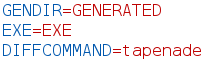
\includegraphics[scale=0.7]{code/var.png}\\
\begin{tabular}{lll}
\verb!GENDIR!&:& dossier où l'ensemble des fichiers générés (.o .f) vont être localisés.\\
\verb!EXE!&:& dossier où se trouvent les fichiers d'exécutions \\
&&Ces deux dossiers permettent de faciliter le make clean.\\
\verb!DIFFCOMMAND!&:& correspond au compilateur tapenade; il doit être installé localement \\
\end{tabular}

Les options de compilations sont données par :\\
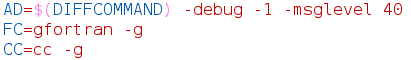
\includegraphics[scale=0.7]{code/flags.png}\\
% \verb!FILE=trig!\\
% Nom du fichier que l'on traite actuellement. \\


% \verb!$(GENDIR)/$(FILE).o : $(FILE).f!\\
% \verb!	$(FC) -c $^  -o $@!\\






La commande principale qui génère l'ensemble des fichiers et qui compile une routine 
main appelant l'ensemble des dérivées est :\\
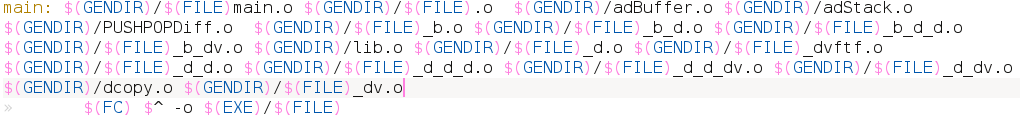
\includegraphics[scale=0.6]{code/main.png}


Afin de pouvoir stocker les variables lors d'un snapshot, Tapenade utilise une librairie
ADFirstAidKit qui g\`ere les piles, d'où les fichiers 
\verb!PUSHPOPDiff, adBuffer, adStack!.

% \noindent
% \verb!$(GENDIR)/PUSHPOPDiff.o : ADFirstAidKit/PUSHPOPDiff.f!\\
% \verb!	$(FC) -c $^ -o $@!\\
% \verb!$(GENDIR)/adBuffer.o : ADFirstAidKit/adBuffer.f!\\
% \verb!	$(FC) -c $^ -o $@!\\
% \verb!$(GENDIR)/adStack.o : ADFirstAidKit/adStack.c!\\
% \verb!	$(CC) -c $^ -o $@!\\

{\tt \_b} signifie que l'on a appliqué le mode inverse, {\tt \_d} le mode direct et {\tt \_dv} le mode multi-directionnel.
Observons maintenant les méchanismes de ces différents modes.

\paragraph{Mode tangent} \hfill \\

Pour rappel, la fonction poss\`ede l'en-tête suivant : \\
     {\tt SUBROUTINE  NOMFONCTION( x, n, f, m, ftf, fj, lfj, g, mode)} \\

Afin d'obtenir le mode tangent par rapport à {\tt g}, il faut exécuter : \\

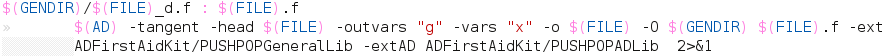
\includegraphics[scale=0.7]{code/tangent.png}

\begin{tabular}{lll}
\verb!-tangent!&:& spécifie de différentiation avec le mode tangent \\
\verb!-head $(FILE)!&:& la routine à traiter porte le nom de la fonction et du fichier \\
\verb!-outvars "g"!&:& variable de sortie \\
\verb!-vars "x"!&:& variable d'entrée \\
\verb!-o $(FILE)!&:& en-tête du nom de fichier généré \\
\verb!-O $(GENDIR) $(FILE).f!&:& place le fichier généré dans le dossier \verb!$(GENDIR)! et\\
 && \verb!$(FILE).f! est le fichier à compiler \\
\end{tabular}

% \noindent
% \verb!$(GENDIR)/$(FILE)_d.f : $(FILE).f!\\
% \verb!	$(AD) -tangent -head $(FILE) -outvars "g" -vars "x" -o $(FILE) -O $(GENDIR)!\\
% \verb! $(FILE).f -ext ADFirstAidKit/PUSHPOPGeneralLib -extAD ADFirstAidKit/PUSHPOPADLib  2>&1!\\

Le fichier \verb!$(FILE)_d.f! est généré dans le dossier GENERATED, cependant il rajoute certaines lignes d'avertissement : \\


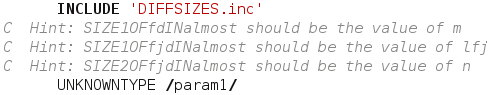
\includegraphics[scale=0.7]{code/tangentajout.png}
% \verb!      INCLUDE 'DIFFSIZES.inc'!\\
% \verb!      UNKNOWNTYPE /param1/!\\
% \verb!C  Hint: SIZE1OFfdINrose should be the value of m!\\
% \verb!C  Hint: SIZE1OFfjdINrose should be the value of lfj!\\
% \verb!C  Hint: SIZE2OFfjdINrose should be the value of n!\\


Ainsi, on supprime les deux lignes contenant \verb!DIFFSIZES! et \verb!UNKNOWNTYPE!
 et on substitue \verb!SIZE*OF*INrose! par les bonnes variables dans le fichier
 grâce à sed.

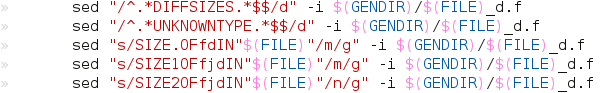
\includegraphics[scale=0.7]{code/tangenttrans.png}

% \noindent
% \verb!	sed "/^.*DIFFSIZES.*$$/d" -i $(GENDIR)/$(FILE)_d.f!\\
% \verb!	sed "/^.*UNKNOWNTYPE.*$$/d" -i $(GENDIR)/$(FILE)_d.f!\\
% \verb!	sed "s/SIZE.OFfdIN"$(FILE)"/m/g" -i $(GENDIR)/$(FILE)_d.f!\\
% \verb!	sed "s/SIZE1OFfjdIN"$(FILE)"/m/g" -i $(GENDIR)/$(FILE)_d.f!\\
% \verb!	sed "s/SIZE2OFfjdIN"$(FILE)"/n/g" -i $(GENDIR)/$(FILE)_d.f!\\

Le fichier \verb!$(GENDIR)/$(FILE)_d.f! est produit et contient l'en-tête : \\
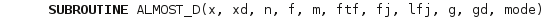
\includegraphics[scale=0.7]{code/tangentent.png}\\
% {\tt SUBROUTINE NOMFONCTION\_D(x, xd, n, f, m, ftf, fj, lfj, g, gd, mode)} \\

Pour comprendre à quoi correspondent les nouvelles variables voici les calculs 
théoriques des résultats. Bien entendu, le produit de la matrice jacobienne avec le
vecteur n'est pas pas calculée en entier.\\


$\left( 
\begin{array}{c} 
\dot{y_1} \\
\dot{y_2} \\
\vdots \\
\dot{y_m}

\end{array}
\right)
=dY = J \times dX =
\underbrace{
\left( 
\begin{array}{ccccc} 
\frac{\partial y_1}{\partial x_1} & \frac{\partial y_1}{\partial x_2} &
 \frac{\partial y_1}{\partial x_3} & \cdots & \frac{\partial y_1}{\partial x_m} \\
\frac{\partial y_2}{\partial x_1} & \frac{\partial y_2}{\partial x_2} &
 \frac{\partial y_2}{\partial x_3} & \cdots & \frac{\partial y_2}{\partial x_m} \\
\vdots & \vdots & \vdots & \ddots & \vdots \\
\frac{\partial y_n}{\partial x_1} & \frac{\partial y_n}{\partial x_2} &
 \frac{\partial y_n}{\partial x_3} & \cdots & \frac{\partial y_n}{\partial x_m} \\
\end{array}
\right)}_{\text{Jacobienne de {\tt g} c'est-à-dire le hessien}}
 \times
\left( 
\begin{array}{c} 
\Tilde{x_1} \\
\Tilde{x_2} \\
\vdots \\
\Tilde{x_m}
\end{array}
\right)
 $ \\
$\Longrightarrow$ {\tt gd} = $\nabla^2 f(x)\times$ {\tt xd} 




 {\tt xd} vecteur $\left(\begin{array}{cccc} 
\Tilde{x_1} &
\Tilde{x_2} &
\hdots &
\Tilde{x_m}
\end{array}\right)^T$


Ainsi, pour calculer {\tt gd}$=\nabla^2f(x)\cdot d$, il suffira d'initialiser la variable {\tt xd}$=d$ et utiliser
les mêmes paramètres que l'appel à la fonction standard.
% $\frac{dg}{dx}xd$



\paragraph{Mode multidirectionnel} \hfill \\

Il s'agit du même procédé que pour le mode tangent mais au lieu d'appliquer un vecteur sur la matrice jacobienne,
on multiplie par une matrice. Par exemple, pour obtenir $\nabla f(x)$, en appliquant le mode multi-directionnel
sur {\tt ftf}, on mutliplie sa jacobienne (c'est-à-dire le gradient) par la matrice identité. Cela revient à appliquer
$n$ fois le mode tangent.\\
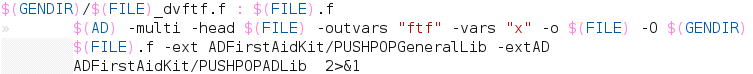
\includegraphics[scale=0.7]{code/multi.png}

Le fichier produit contient l'en-tête suivant :\\
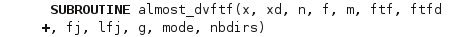
\includegraphics[scale=0.7]{code/multient.png}
% {\tt   SUBROUTINE NOMDEFONCTION\_dvftf(x, xd, n, f, m, ftf, ftfd
%      +, fj, lfj, g, mode, nbdirs)}\\

En revanche cette fois-ci, {\tt xd} $\in \mathbb{R}^{n\times n}$
et {\tt nbdirs} nombre de directions voulues {\tt nbdirs=n}


\paragraph{Mode inverse} \hfill \\

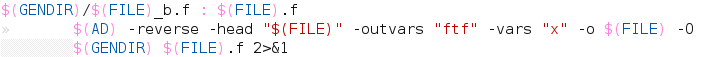
\includegraphics[scale=0.7]{code/inverse.png}\\
\begin{tabular}{lll}
Variable d'entrée&:& {\tt x} \\
Variable de sortie&:& {\tt ftf} \\
\end{tabular}
% Variable de sortie : ftf\\
% Variable d'entrée : x\\

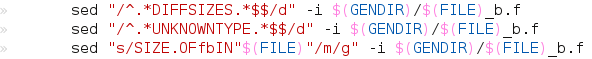
\includegraphics[scale=0.7]{code/inversetrans.png}\\

\`A partir de la fonction :\\
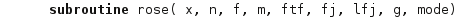
\includegraphics[scale=0.7]{code/entete.png}\\
% {\tt SUBROUTINE  NOMFONCTION( x, n, f, m, ftf, fj, lfj, g, mode)} \\
en dérivant ftf par rapport à x en mode inverse nous obtenons\\
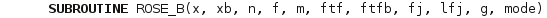
\includegraphics[scale=0.7]{code/inverseent.png}\\

$\left( 
\begin{array}{c} 
\bar{x_1} \\
\bar{x_2} \\
\vdots \\
\bar{x_m}

\end{array}
\right)
=dX = J^* \times dY = \left( 
\begin{array}{ccccc} 
\frac{\partial y_1}{\partial x_1} & \frac{\partial y_2}{\partial x_1} &
 \frac{\partial y_3}{\partial x_1} & \cdots & \frac{\partial y_n}{\partial x_1} \\

\frac{\partial y_1}{\partial x_2} & \frac{\partial y_2}{\partial x_2} &
 \frac{\partial y_3}{\partial x_2} & \cdots & \frac{\partial y_n}{\partial x_2} \\

\vdots & \vdots & \vdots & \ddots & \vdots \\

\frac{\partial y_1}{\partial x_m} & \frac{\partial y_2}{\partial x_m} &
 \frac{\partial y_3}{\partial x_m} & \cdots & \frac{\partial y_n}{\partial x_m} \\
\end{array}
\right) \times
\left( 
\begin{array}{c} 
\bar{y_1} \\
\bar{y_2} \\
\vdots \\
\bar{y_m}

\end{array}
\right)
 $ \\ 

 $\Longrightarrow$ {\tt xb} = $\nabla f(x)^T\times$ {\tt ftfb} $= \nabla f(x)^T\times[1] = \nabla f(x)^T$


Dans notre cas, puisque {\tt ftf} est un scalaire, la matrice Jacobienne n'a qu'une seule colonne et {\tt ftfb}
est un scalaire.






